\section{Base di Dati}
    \subsection{Scelta delle tabelle}

    Si è implementato un database in SQL per gestire tutti i dati inseriti dagli utenti e dagli amministratori.
    Di seguito sono elencate le tabelle utilizzate e i campi degni di nota:
    \begin{itemize}
        \item \textbf{ Articolo}: contiene le notizie da pubblicare nel sito e un url locale per accedere alle foto salvate da pubblicare;
        \item \textbf{ Biglietto}: contiene i biglietti acquistati;
        \item \textbf{ Partita}: presenta i dati relativi alla partita, tra cui i costi dei biglietti e il risultato;
        \item \textbf{ Posto}: indica i settori dello stadio;
        \item \textbf{ Squadra}: contiene i dati relativi alle squadre;
        \item \textbf{ Stadio}: contiene i dati relativi agli stadi;
        \item \textbf{ Utente}: colleziona i dati di ogni utente registrato; il campo “password” è criptato e il campo “livello\_privilegi” differenzia gli utenti dagli amministratori.
    \end{itemize}
    
    \begin{center}
        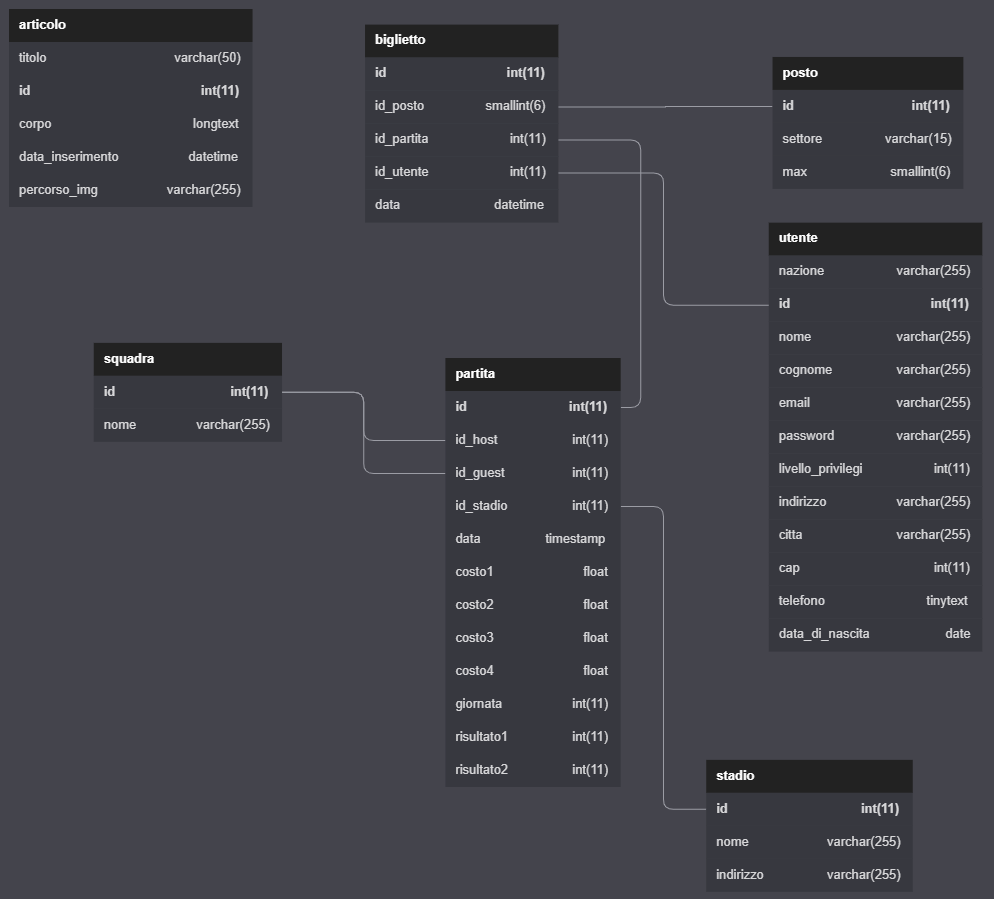
\includegraphics[scale=0.5]{images/database.png}
    \end{center}
    
    \subsection{Identificatori primari}
    Ogni tabella del database ha un attributo denominato "id", che fornisce un identificatore unico per ogni record delle tabelle; tale attributo è utilizzato come chiave primaria per gestire tutte le relazioni fra le tabelle.
    \subsection{Chiavi Esterne}
    Sono state utilizzate le seguenti relazioni:
    \begin{itemize}
        \item La tabella Biglietto utilizza come chiavi esterne, le chiavi primarie di Posto, Partita e Utente;
        \item La tabella Partita utilizza come chiavi esterne, le chiavi primarie di Squadra e Stadio.
    \end{itemize}

    \subsection{Forma normale}
    Il database è stato pensato e realizzato in forma normale per evitare ridondanza informativa e il rischio di incoerenza dei dati.
    
    \subsection{Utilizzo atteso}
    Il database è stato progettato per rispondere alle seguenti esigenze:
    \begin{itemize}
        \item Gestire gli utenti, permettendo loro di registrati al sito e gli amministratori;
        \item Tenere traccia delle partite delle squadre di calcio;
        \item Consentire l’acquisto dei biglietti delle partite giocate nello stadio Torre Archimede;
        \item Tenere traccia dei biglietti degli utenti, gestendone gli acquisti e i rimborsi;
        \item Gestire le notizie del sito.
    \end{itemize}

    